\chapter{Results}\label{results}
\section{Experimental Setup}
The experiment executed in this chapter, consists of calculating a baseline measurement, by optimizing threshold $\mathcal{T}$ to find the maximum sentence level F1-score, inserting the external knowledge graph into our pipeline and overriding classifications in the baseline pipeline, hoping to improve the false positives count and error detection rate, resulting in an improved F1-score. 
The dataset we will be performing these experiments on contains 28 sentences which contain a hallucination, which need to be labelled \texttt{INCORRECT}, and 19 that are factual (\texttt{CORRECT}), the distribution can be found in Table \ref{tab:sentence_ground_truth_distribution}. The distribution of claims can be found in Table \ref{tab:atomic_label_distribution}. 

\begin{table}[ht]
    \centering
    \caption{Distribution of ground truth labels in the binary sentence dataset.}
    \label{tab:sentence_ground_truth_distribution}
    \begin{tabular}{lcc}
        \toprule
        \textbf{Label} & \textbf{Count} & \textbf{Percentage} \\
        \midrule
        INCORRECT (Hallucinated) & 28 & 59.6\% \\
        SUPPORTED (Correct) & 19 & 40.4\% \\
        \midrule
        \textbf{Total} & \textbf{47} & \textbf{100.0\%} \\
        \bottomrule
    \end{tabular}
\end{table}

\section{Baseline NLI Performance}
% summary piece of the section 
In order to score the succes of our experiment, we will first need to set a baseline measurement. This baseline consists of calculating the confidence threshold $\mathcal{T}$ and running the pipeline without inserting external knowledge. 

\subsection{Confidence Threshold Optimization}\label{sec:confidenceT}
To determine the label assigned to an atomic claim in our evaluation module, we use the confidence threshold ($\mathcal{T}$). Before evaluating the baseline pipeline's predictive performance, the optimal confidence threshold ($\mathcal{T}$) was established to maximize the F1-score on the sentence level. We chose to maximize this metric, since the primary objective of the framework is to detect hallucinatinos at the sentence level and optimizing strictly for atomic performance worked counter intuative. 
The results of our threshold optimization can be found in Figure \ref{fig:threshold_optimization}. 

\begin{figure}[ht]
    \centering
    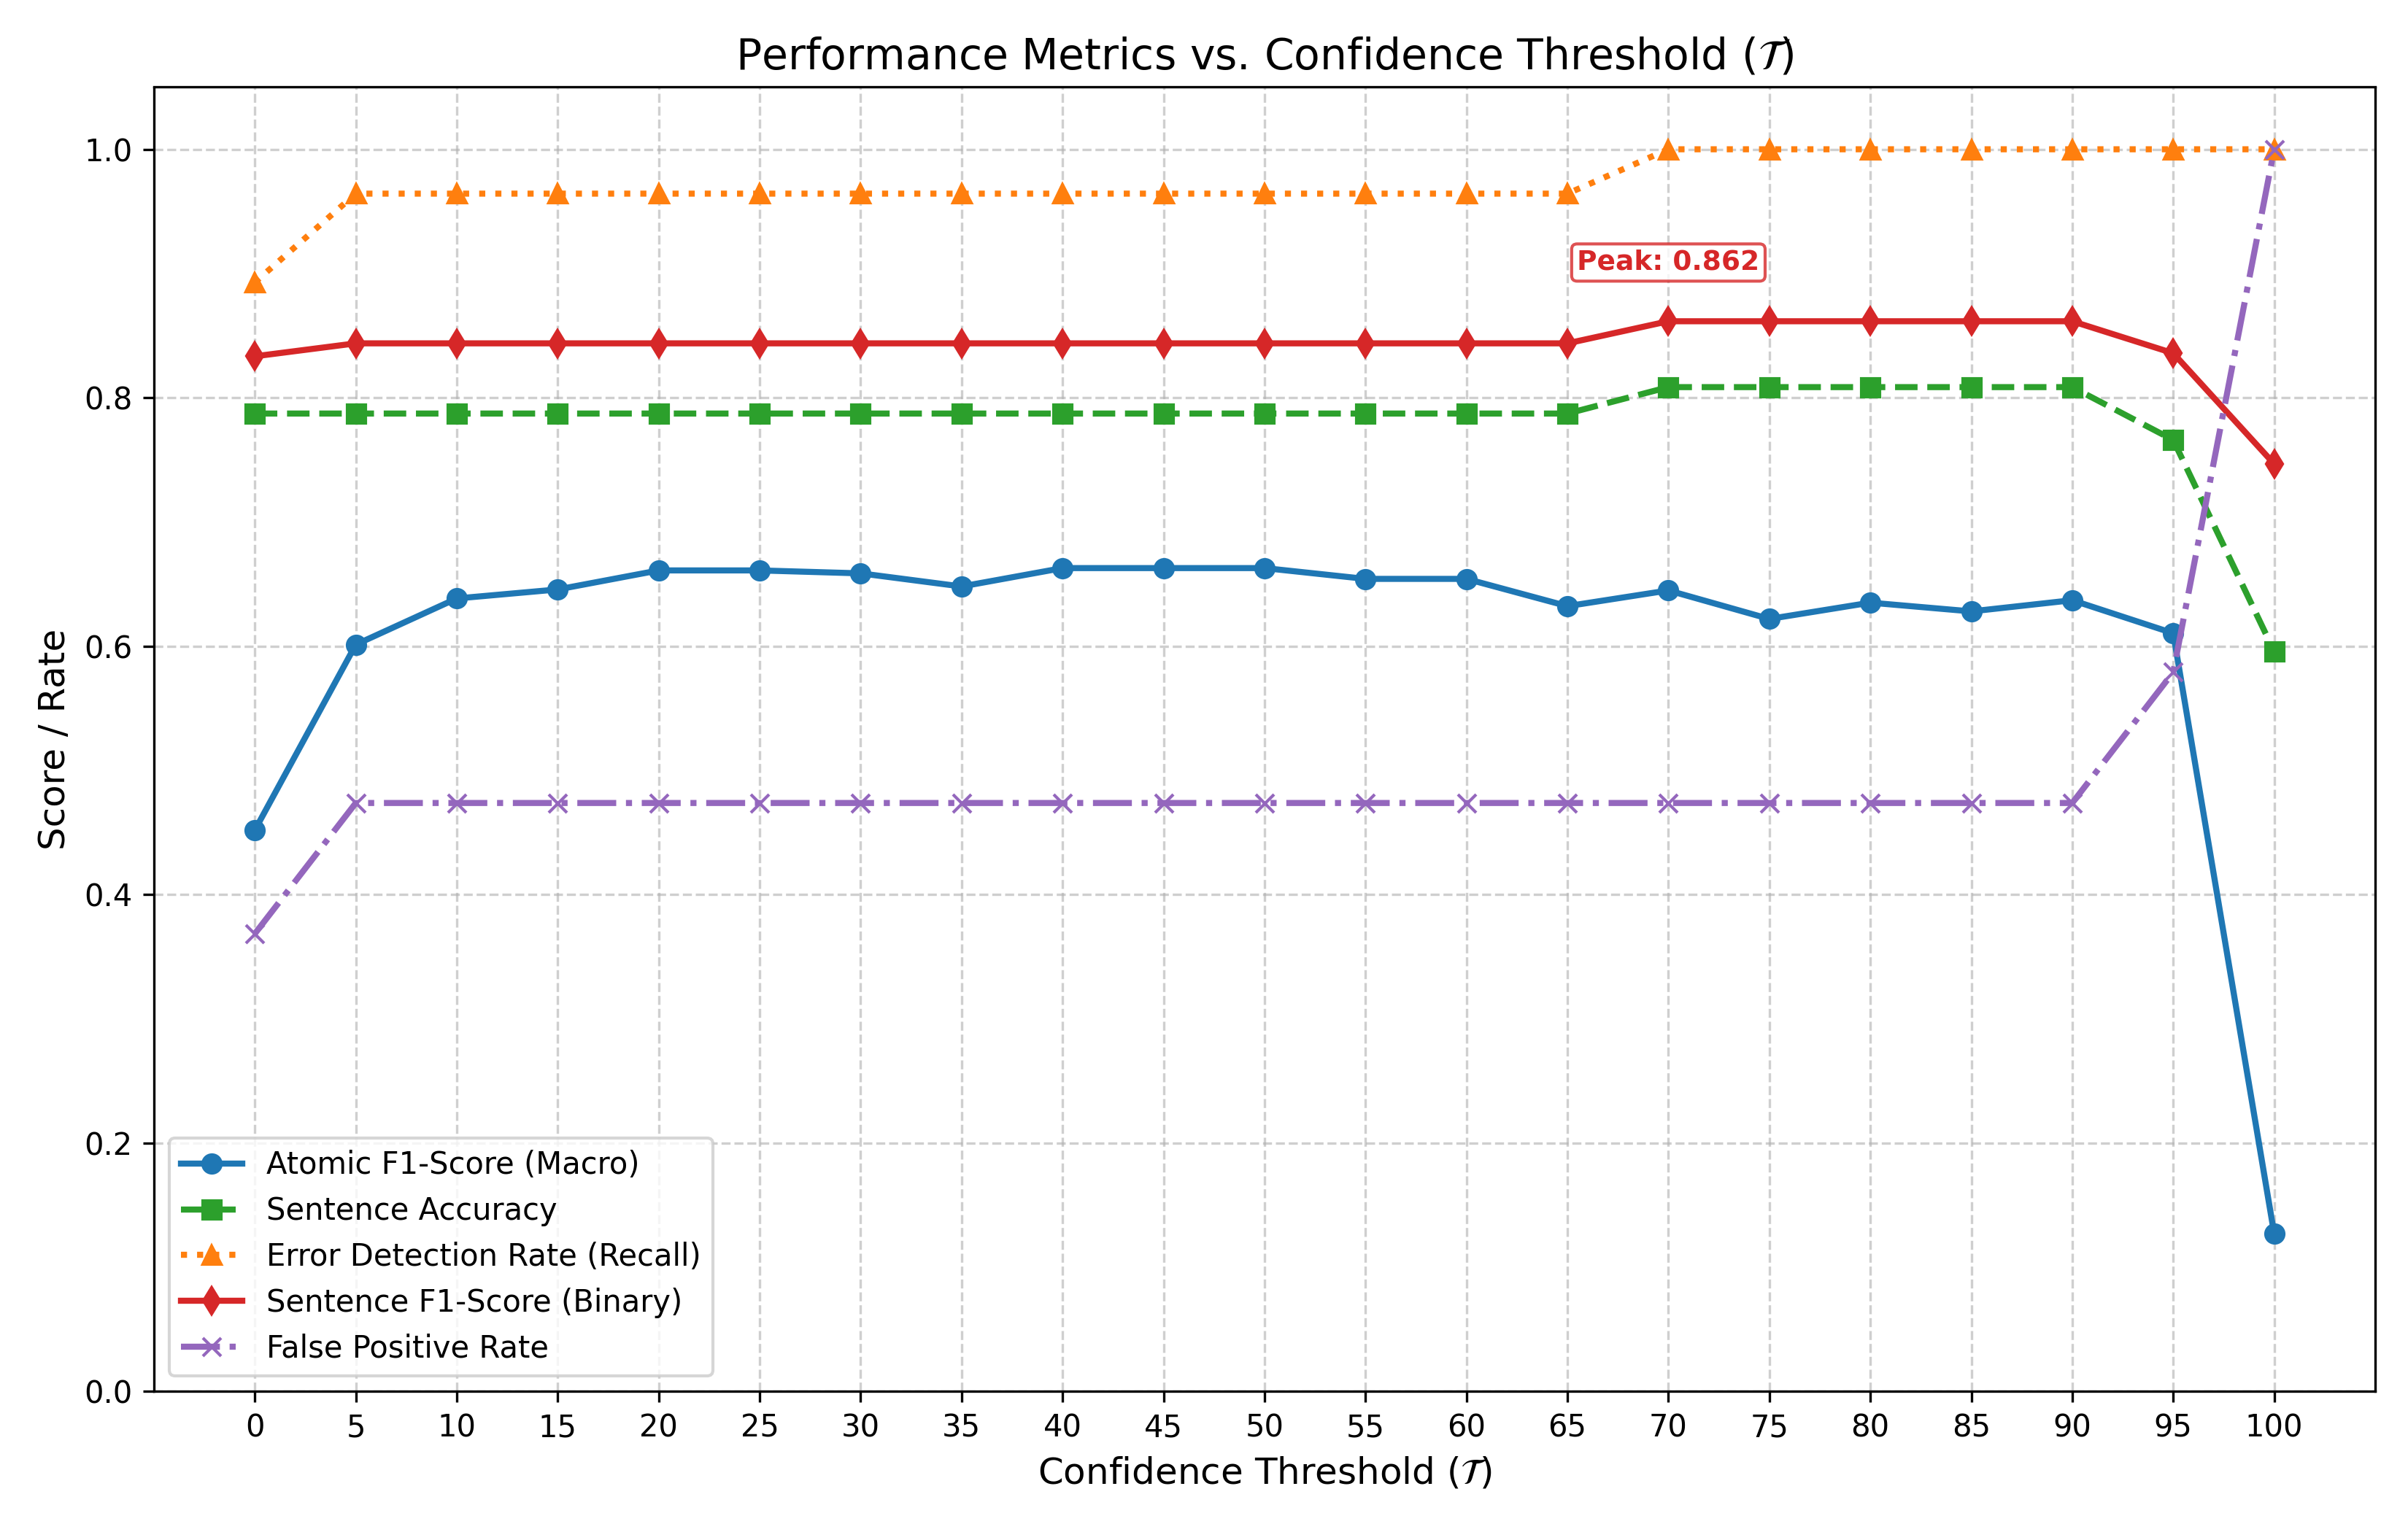
\includegraphics[width=0.9\textwidth]{graphs/threshold_optimization_plot.png}
    \caption{Macro F1-Score plotted against the confidence threshold ($\mathcal{T}$) during the baseline evaluation. The model's predictive performance plateaus at exactly $\mathcal{T} = 0.65$, demonstrating the strict polarization of the XLM-ROBERTa softmax logits.}
    \label{fig:threshold_optimization}
\end{figure}

\noindent Figure \ref{fig:threshold_optimization} shows that the pipeline reaches a maximum F1-score of $0.862$ at $\mathcal{T} = 70.0$. Table \ref{tab:optimal_threshold_metrics} shows the values of all lines at this $\mathcal{T}$ Even though the F1-score of the atomic claims is higher at $\mathcal{T} = 40.0$, the F1 score is higher at 70 due to the error detection rate being 1.0, entailing that every error was found correctly, and the accuracy reaching 0.8085. The high threshold does introduce a False Positive Rate of $0.4737$ at the sentence level, but this rate is constant from thresholds ranging from $5$ untill $90$. 
\begin{table}[htbp]
    \centering
    \caption{Performance Metrics at Optimal Sentence-Level Threshold ($\mathcal{T} = 70.0$)}
    \label{tab:optimal_threshold_metrics}
    \begin{tabular}{lcc}
        \toprule
         \textbf{Level} & \textbf{Metric} & \textbf{Score} \\
        \midrule
        Sentence & F1-Score & $0.8615$ \\
        Atomic & F1-Score (Macro) & $0.6448$ \\
        Sentence & Accuracy & $0.8085$ \\
        Sentence & Error Detection Rate (Recall) & $1.0000$ \\
        Sentence & False Positive Rate & $0.4737$ \\
        \bottomrule
    \end{tabular}
\end{table}

\noindent These flat scores directly follow from the distribution of confidence scores generated by the \rob baseline. As seen in Figure \ref{fig:score_distribution}, the model exhibits a confidence distribution where the vast majority of assigned scores cluster at the extremes ($\ge 90\%$ or $\le 20\%$)  Because the model rarely outputs intermediate confidence scores, adjusting the threshold within this massive section band doesn't lead to a significant number of claims receiving a different classification. This behavior also explains why the variance between the lowest and highest possible F1-Scores across the non-extreme ($90 \le \mathcal{T} \le 20$) threshold range is a difference of only $0.04$ (approximately $4\%$).

For our other calculations, $\mathcal{T} =70$ was selected. Since the metrics did not improve after this  $\mathcal{T}$ and by increasing the threshold we increase the possibility of our modelling being prone to be overfitted. 

\begin{figure}[ht]
    \centering
    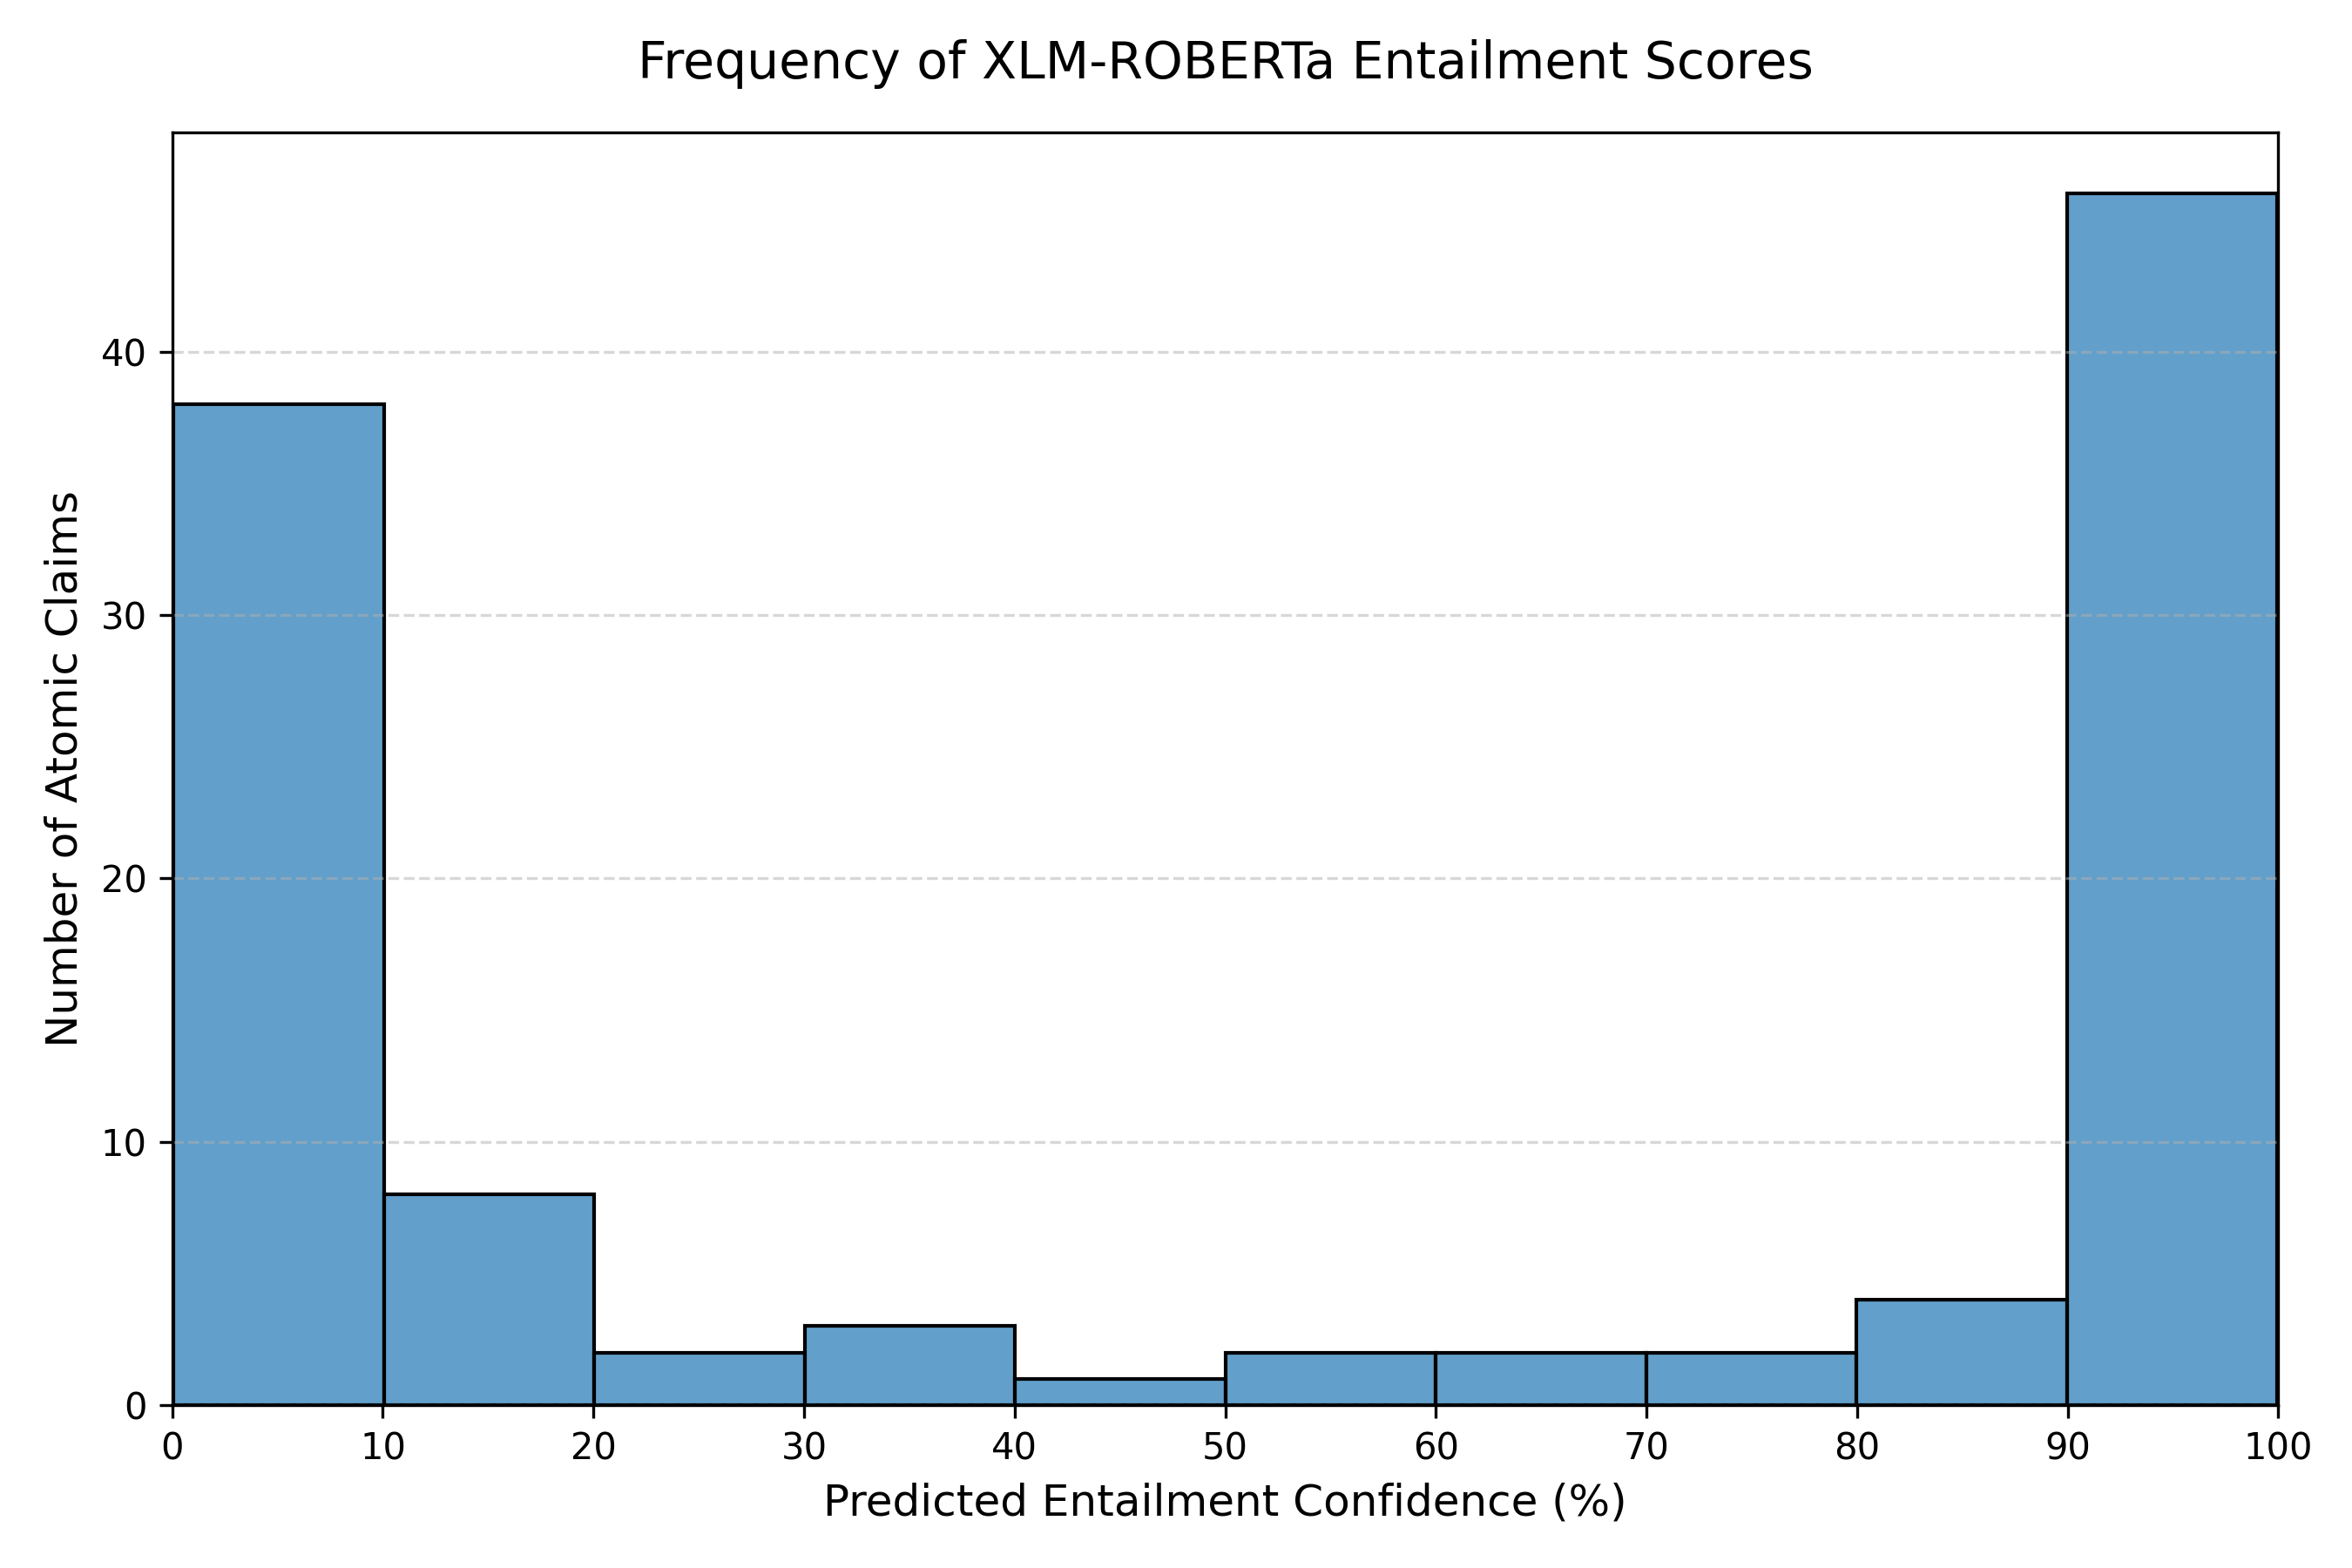
\includegraphics[width=0.8\textwidth]{graphs/score_histogram_plot.png}
    \caption{Histogram showing the distribution of model entailment confidence across all atomic claims. The bimodal pattern confirms that the majority of predictions are polarized toward total certainty or total uncertainty.}
    \label{fig:score_distribution}
\end{figure}


\subsection{Atomic Claim Level Performance}
The baseline performance of the \rob model at the atomic claim level allows us to look at the system's ability to assign the \texttt{SUPPORTED}, \texttt{INTRINSIC} and \texttt{EXTRINSIC} labels. As summarized in Table \ref{tab:baseline_atomic_metrics}, the model achieved a Macro F1-Score of 0.526, with a Precision of 0.737 and a Recall of 0.601. These metrics indicate that the model scores well on the task of identifying claims that are supported by the source, but has a lower accuracy on labelling the intrinsic and extrinsic hallucinations. 

\begin{table}[htbp]
    \centering
    \caption{Performance Metrics at Optimal Sentence-Level Threshold ($\mathcal{T} = 70.0$)}
    \label{tab:baseline_atomic_metrics}
    \begin{tabular}{lc}
        \toprule
        \textbf{Metric} & \textbf{Score} \\
        \midrule
        F1-Score (Macro) &    0.6448 \\ 
        Accuracy &            0.7653 \\ 
        Error Detection &     0.8837 \\ 
        False Positive &      0.3273 \\ 
        \bottomrule
    \end{tabular}
\end{table}
  


\noindent To understand the model's classification errors, the confusion matrix in Figure \ref{fig:baseline_confusion_matrix}  shows the distribution of our predictions across the three atomic labels. Due to the data set containing 51\% of claims that are labelled \texttt{SUPPORTED} in our ground truth (Table \ref{tab:ground_truth_distribution}), the matrix shows the most values for the supported labels. The model marked 12 \texttt{SUPPORTED} claims as \texttt{INTRINSIC}, this backs up the False Positive numbers we encountered. 

\begin{figure}[ht]
    \centering
    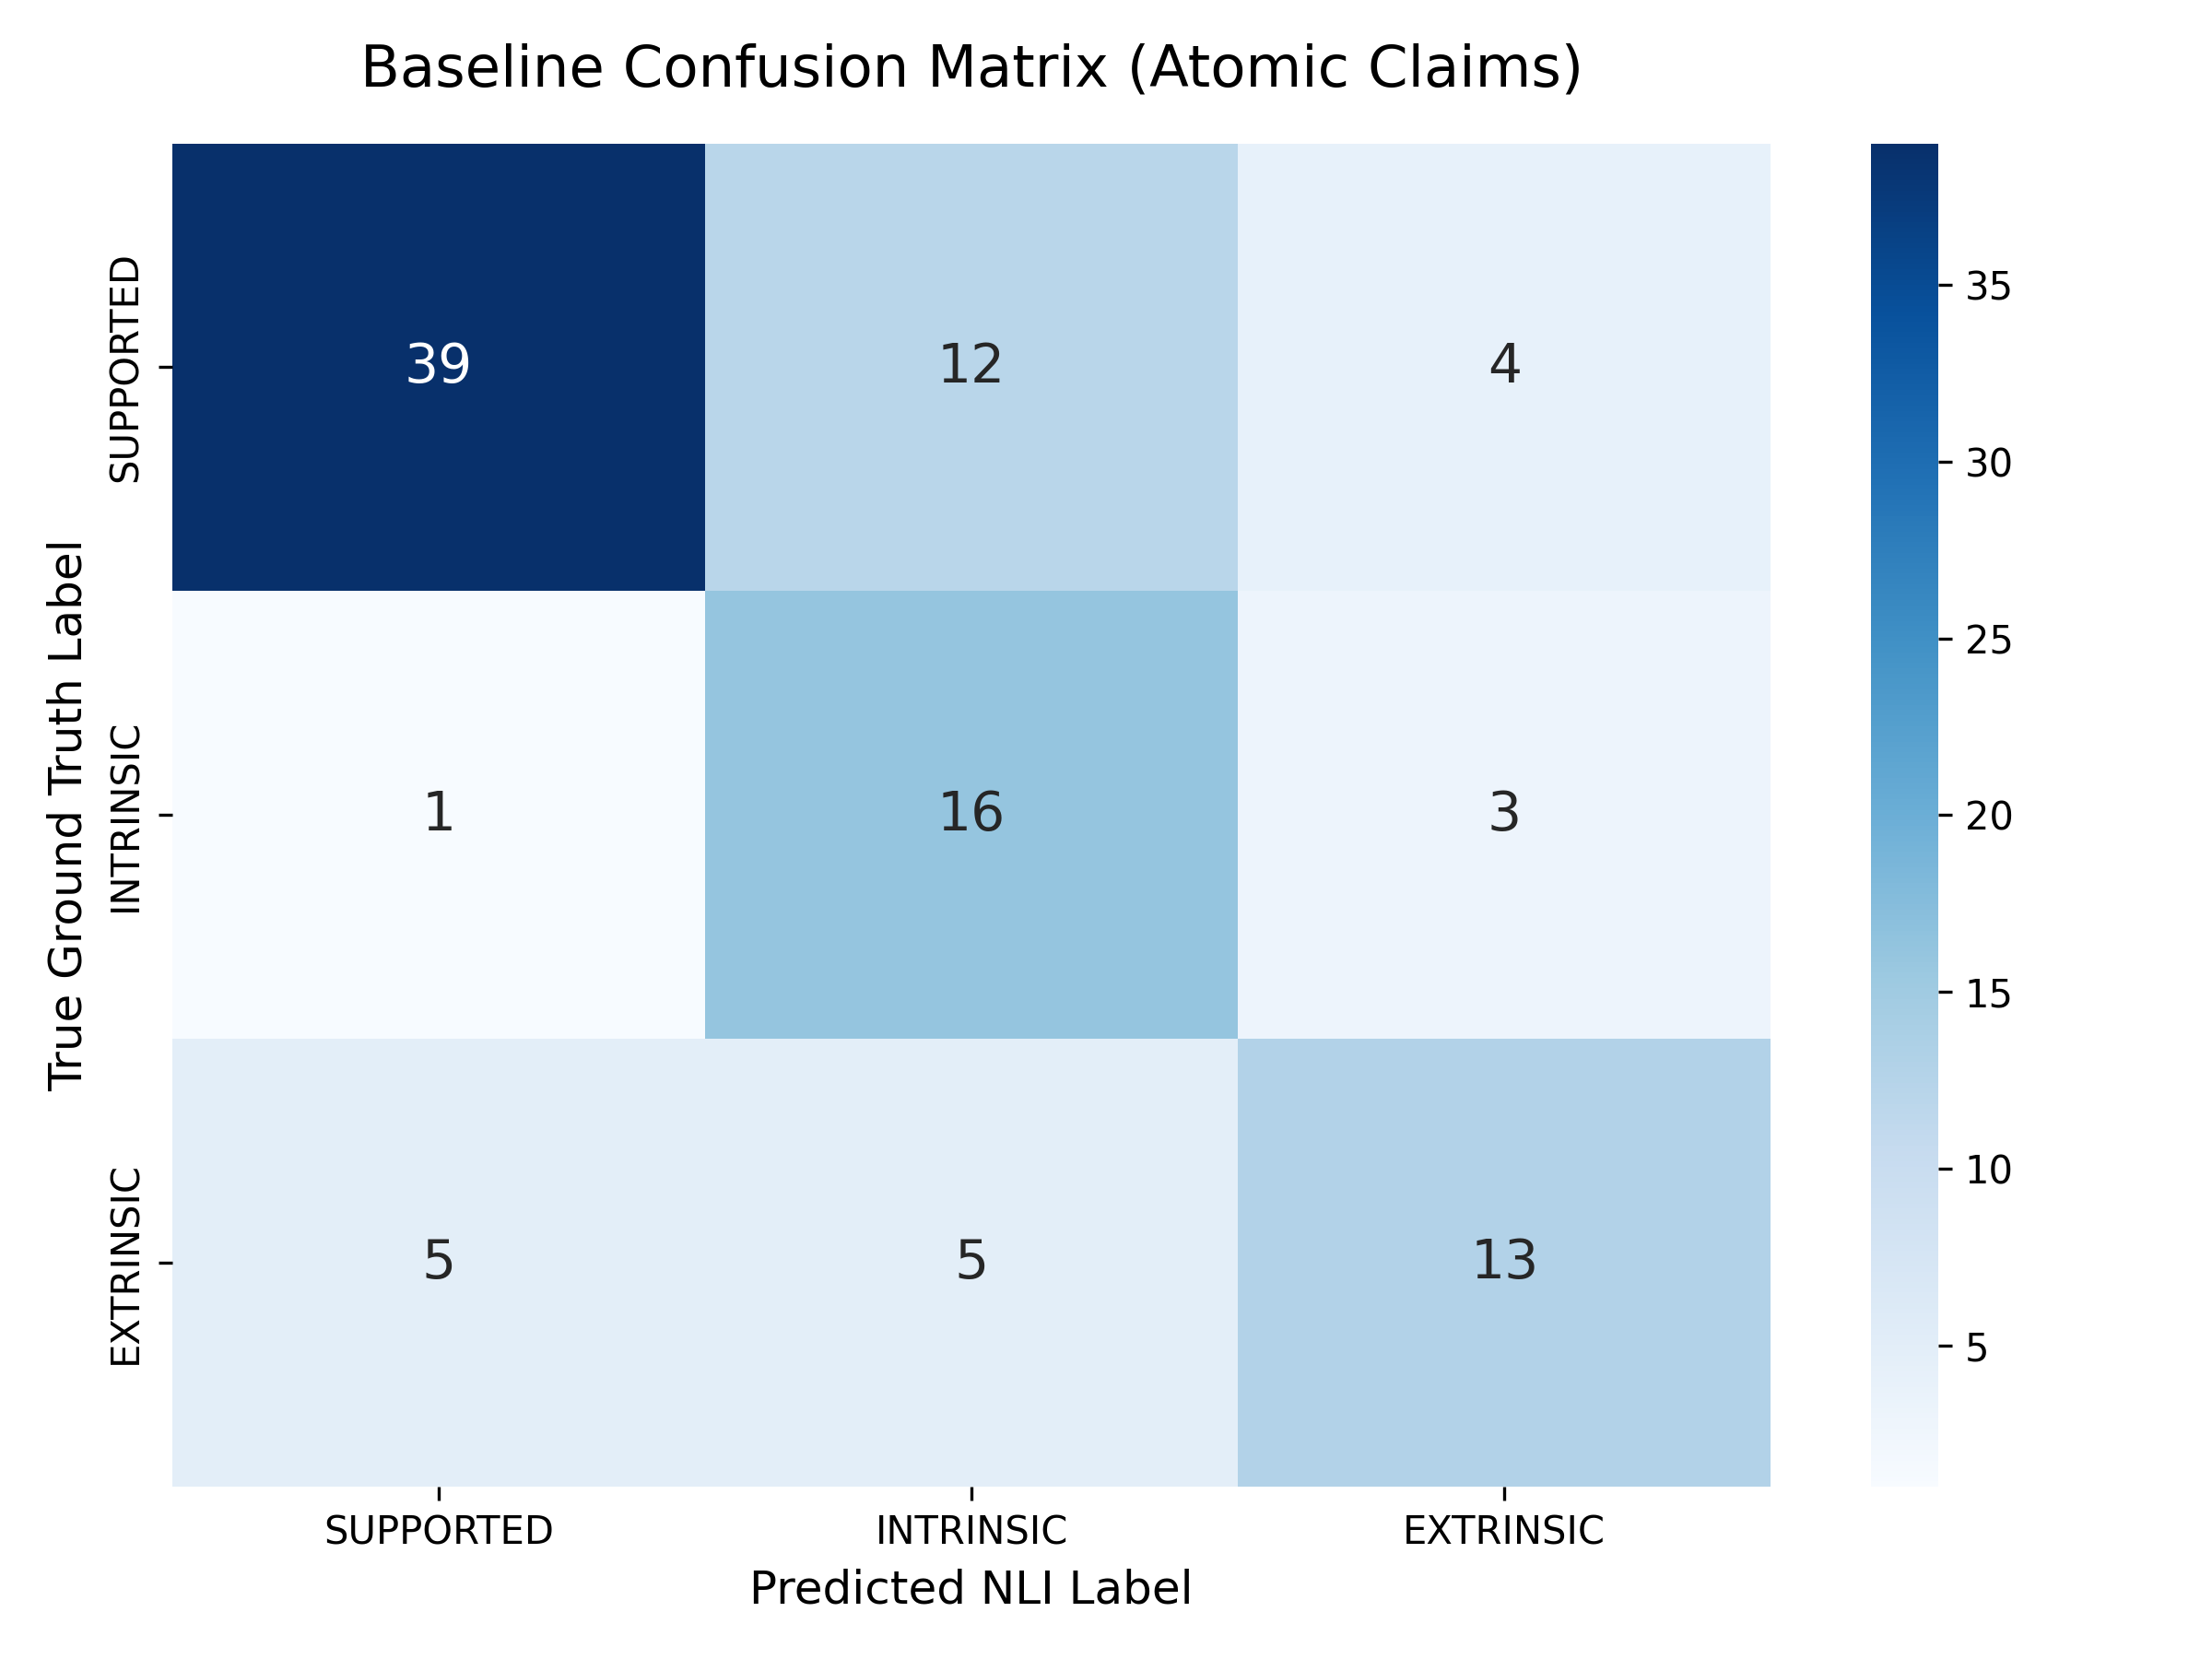
\includegraphics[width=0.8\textwidth]{graphs/baseline_confusion_matrix.png}
    \caption{Confusion matrix of the baseline XLM-ROBERTa model at the atomic claim level. The heatmap illustrates the model's distribution of predictions across the three label categories. The significant misclassification of 'EXTRINSIC' hallucinations as 'SUPPORTED' underscores the model's tendency to conflate high lexical overlap with factual entailment.}
    \label{fig:baseline_confusion_matrix}
\end{figure}

\begin{table}[ht]
    \centering
    \caption{Distribution of Ground Truth vs. Predicted labels in the atomic claim dataset at Baseline ($\mathcal{T} = 70.0$).}
    \label{tab:atomic_label_distribution}
    \begin{tabular}{lcccc}
        \toprule
        & \multicolumn{2}{c}{\textbf{Ground Truth}} & \multicolumn{2}{c}{\textbf{Predicted (Baseline)}} \\
        \cmidrule(lr){2-3} \cmidrule(lr){4-5}
        \textbf{Label} & \textbf{Count} & \textbf{Percentage} & \textbf{Count} & \textbf{Percentage} \\
        \midrule
        SUPPORTED & 55 & 56.1\% & 42 & 42.9\% \\
        EXTRINSIC & 24 & 24.5\% & 25 & 25.5\% \\
        INTRINSIC & 19 & 19.4\% & 31 & 31.6\% \\
        \midrule
        \textbf{Total} & \textbf{98} & \textbf{100.0\%} & \textbf{98} & \textbf{100.0\%} \\
        \bottomrule
    \end{tabular}
\end{table}

Taking a dive into these misclassifications, this trend continues. For example, when analysing the `Daryll-Ann Weeps' entry (Table \ref{tab:daryll_ann_scores}), the claim C.3, was predicted as \\ \texttt{INTRINSIC}, while the claim actually holds, but no sentence noted this exact claim, which is why the low entailment score was generated. The evidence for this contradiction was a sentence which explained that the band recorded the album thirty years ago, which \rob sees as a contradiction because they won't be performing it for the first time according to that sentence. 
% "evidence_used": "Over Daryll-Ann: De Nederlands gitaarpopband Daryll-Ann nam dertig jaar geleden het album 'Daryll-Ann Weeps' op.",

\begin{table}[htbp]
    \vspace{0.2cm}
    \begin{flushleft}
        \textbf{C.3:} \textit{The Dutch guitar pop band performs their cult-classic album `Daryll-Ann Weeps' for the first time}
    \end{flushleft}
    \vspace{-0.3cm} % Trek de tabel iets dichter naar de claim toe
    \centering
    \label{tab:daryll_ann_scores}
    \begin{tabular}{lc}
        \toprule
        \textbf{NLI Metric} & \textbf{Confidence Score (\%)} \\
        \midrule
        Entailment (\texttt{best\_ent\_score}) & $5.0178$ \\
        Contradiction (\texttt{best\_con\_score}) & $99.0805$ \\
        \bottomrule
    \end{tabular}
    \caption{Raw NLI Confidence Scores for the Analyzed Claim}
\end{table}


\subsection{Sentences}
Using the min aggregation method from Section \ref{rsh:eval}, we are able to use the threshold $\mathcal{T = 70.0}$ to classify sentences as either \texttt{CORRECT} or \texttt{INCORRECT}. 

In Table \ref{tab:baseline_binary_metrics}, the final baseline metrics can be found. We will use these values as a baseline to check our experiment against. Notable is that no False Negatives were found, meaning that we did manage to detect every sentence with a hallucination. However, this does come with the downside of our False Positive Rate reaching 0.4737, meaning that our baseline model flags almost half of verifiable sentences as a hallucination. 

\begin{table}[htbp]
    \centering
    \caption{Baseline performance metrics aggregated at the sentence level.}
    \label{tab:baseline_binary_metrics}
    \begin{tabular}{lc}
        \toprule
        \textbf{Metric} & \textbf{Score} \\
        \midrule
        F1-Score         &    0.8615 \\ 
        Accuracy &            0.8085 \\ 
        Error Detection &     1.0000 \\ 
        False Positive &      0.4737 \\ 
        \bottomrule
    \end{tabular}
\end{table}


\begin{figure}[ht]
    \centering
    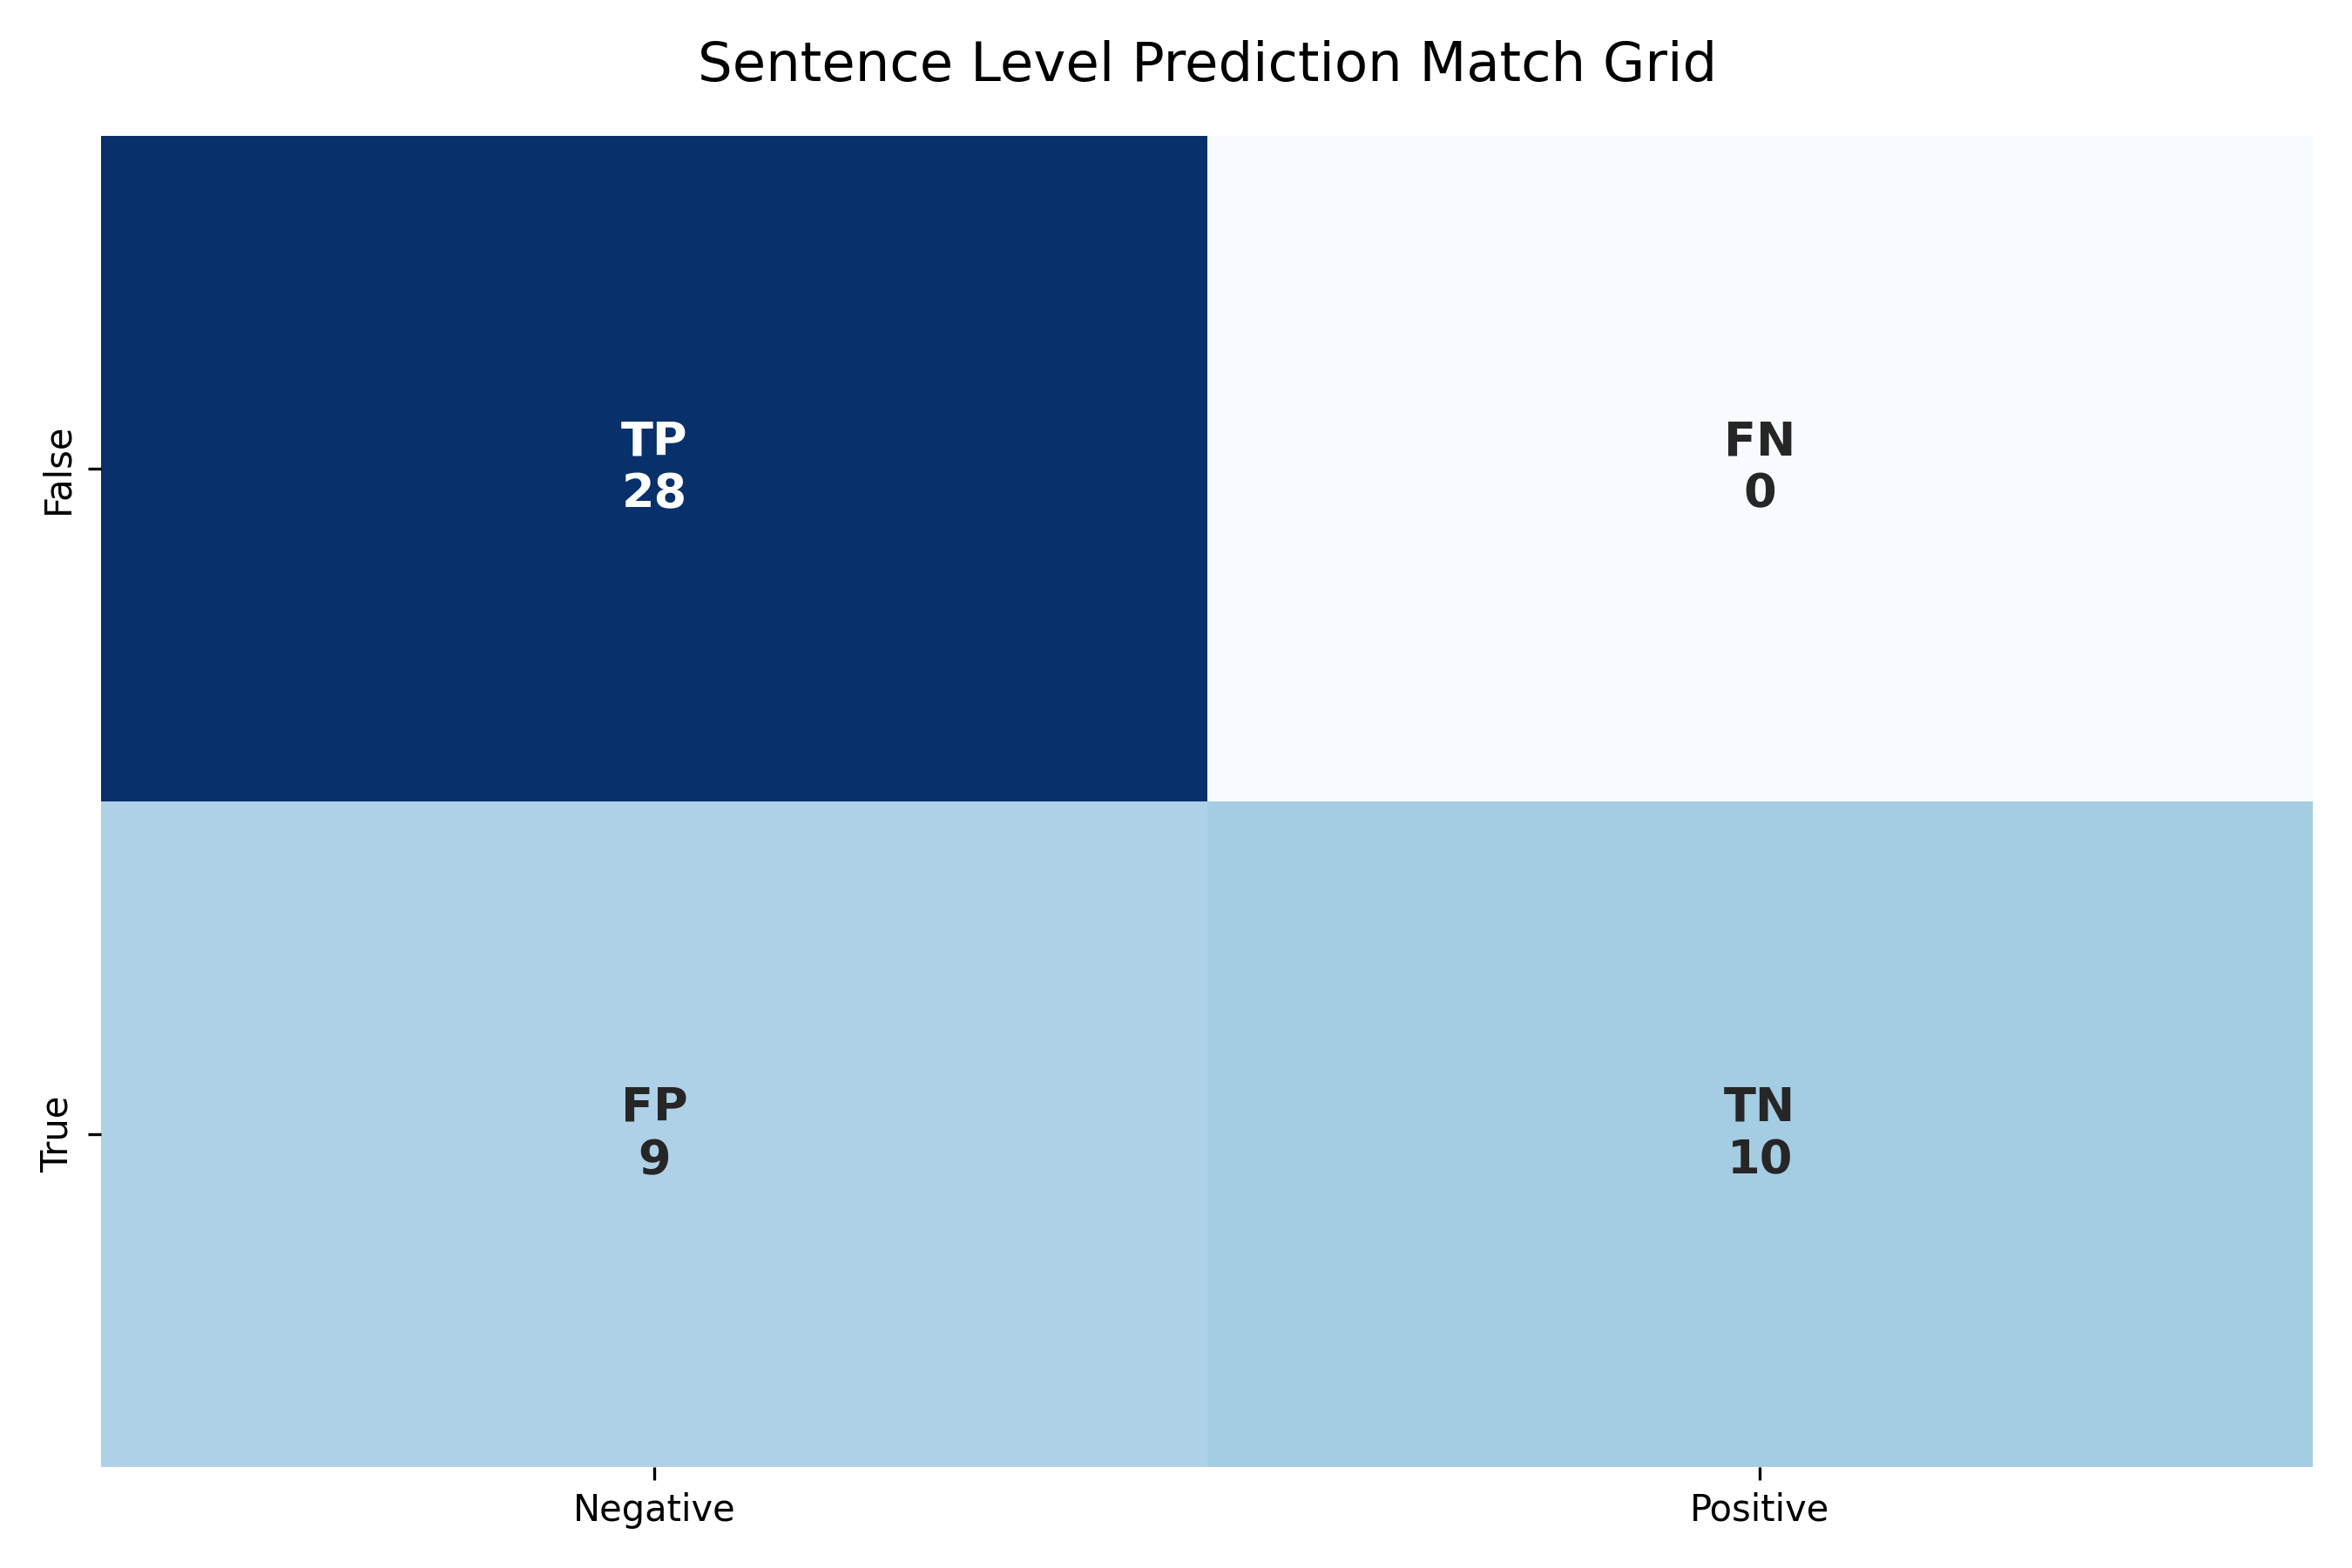
\includegraphics[width=0.8\textwidth]{graphs/baseline_prediction_match_grid.png}
    \caption{.}
    \label{fig:threshold_optimization}
\end{figure}


\section{Experimental Setup}
The goal of the experimental set up is to test if injecting the MusicBrainz data, an external knowledge graph, can improve the models performance, based on the baseline sentence level F1-score (0.8615) and the baseline false positives rate (0.4737). During the baseline set up, the confidence threshold of $\mathcal{T} = 70.0$ was established and will be used for our calculations, to ensure that both pipelines are identical apart from the addition of the knowledge graph. 

The knowledge graph is able to insert data ranging over the following topics: \texttt{area}, \texttt{country} and \texttt{genre}, which can be found in Table \ref{tab:mb_synthesis_templates}. In total, 56 claims (see Table \ref{tab:atomic_label_distribution}) were attempted to be overriden, since we only try to change verdicts that are \texttt{INTRINSIC} or \texttt{EXTRINSIC} and the result will either be {INTRINSIC} or \texttt{SUPPORTED}. 

\subsection{Experiment Atomic Claim Level Performance}\label{res:experiment_atomic_claims}
% talk about the overall atomic claim performance and the differences, e.g. some moving, and show a positive change and a negative change. 
At the atomic claim level, the integration of the Knowledge Graph resulted in a shift exclusively within the ternary metrics. As shown in Table \ref{tab:experiment_atomic_metrics}, the Macro F1-Score decreased slightly to 0.6153. This minor decrease occurs because the ternary calculation treats all three labels as distinct categories; moving a claim from one error class to another alters the distribution without improving the binary correct/incorrect ratio. To understand this shift, we examine the specific label overrides.

\begin{table}[htbp]
    \centering
    \caption{Experimental Performance Metrics at Optimal Sentence-Level Threshold ($\mathcal{T} = 70.0$)}
    \label{tab:experiment_atomic_metrics}
    \begin{tabular}{lc}
        \toprule
        \textbf{Metric} & \textbf{Score} \\
        \midrule
        F1-Score (Macro) &    0.6153 \\ 
        Accuracy &            0.7653 \\ 
        Error Detection &     0.8837 \\ 
        False Positive &      0.3273 \\ 
        \bottomrule
    \end{tabular}
\end{table}

As we can see in Table \ref{tab:atomic_label_distribution_experiment}, 5 \texttt{EXTRINSIC} claims have been overwritten to be \texttt{INTRINSIC}. When analysing these claims and the evidence given by the validation module, we can sort them into two categories based on the synthezied sentence type used as evidence. The first 3 claims that were now labelled as contradictions, were regarding the origin of the artist. Table \ref shows C.4, of artist ``Adult DVD''. In the original source text, no origin is mentioned, but our external database showed they are not from The Netherlands, leading to a correct jump to \texttt{INTRINSIC}. 

Table \ref{tab:hybrid_validation_examples} shows C.5 related to artist ``daoud''. The type of evidence used, is based on the genre of music they create, which leads to a contradiction, since ``unconventional, danceable, and cheerful jazz that blends hip-hop grooves'' is not the exact same as ``downtempo, instrumental music''. Table \ref{tab:override_accuracy_summary} shows all 5 shifts and their respective synthezied source category, which leads us to believe our model is more accurate on the artists origin than their music genre. 

  \begin{table}[ht]
    \centering
    \caption{Distribution of Ground Truth vs. Predicted labels in the atomic claim dataset at Experiment ($\mathcal{T} = 70.0$).}
    \label{tab:atomic_label_distribution_experiment}
    \begin{tabular}{lcccc}
        \toprule
        & \multicolumn{2}{c}{\textbf{Ground Truth}} & \multicolumn{2}{c}{\textbf{Predicted (Experiment)}} \\
        \cmidrule(lr){2-3} \cmidrule(lr){4-5}
        \textbf{Label} & \textbf{Count} & \textbf{Percentage} & \textbf{Count} & \textbf{Percentage} \\
        \midrule
        SUPPORTED & 55 & 56.1\% & 42 & 42.9\% \\
        EXTRINSIC & 24 & 24.5\% & 20 & 20.4\% \\
        INTRINSIC & 19 & 19.4\% & \textbf{36} & 36.7\% \\
        \midrule
        \textbf{Total} & \textbf{98} & \textbf{100.0\%} & \textbf{98} & \textbf{100.0\%} \\
        \bottomrule
    \end{tabular}
\end{table}

\begin{table}[htbp]
    \centering
    \caption{Examples of incorrect baseline signals successfully overridden by the Knowledge Graph to an intrinsic contradiction (\texttt{INTRINSIC}).}    \label{tab:hybrid_validation_examples}
    \renewcommand{\arraystretch}{1.3}

    % --- Voorbeeld 1: daoud (Taxonomische frictie) ---
    \vspace{0.2cm}
    \begin{flushleft}
        \textbf{C.4:} \textit{The French-Moroccan trumpeter and composer daoud plays unconventional, \textcolor{red}{danceable, and cheerful} jazz that blends hip-hop grooves}
    \end{flushleft}
    \vspace{-0.3cm} 
    \begin{tabular}{l r r p{0.55\linewidth}}
        \toprule
        \textbf{KG Verdict} & \textbf{Ent. Score} & \textbf{Con. Score} & \textbf{Evidence Used (MusicBrainz)} \\
        \midrule
        CONTRADICTION & 2.36 & 95.19 & \textit{daoud} plays downtempo, instrumental music. \\
        \bottomrule
    \end{tabular}

    \vspace{0.4cm} % Ruimte tussen de twee claims

    % --- Voorbeeld 2: Adult DVD (Geografische frictie) ---
    \begin{flushleft}
        \textbf{C.5:} \textit{Adult DVD, A six-piece synthpunk band from the \textcolor{red}{Netherlands} returns with danceable, retro computer game-like music that grooves, rocks, and swings}
    \end{flushleft}
    \vspace{-0.3cm}
    \begin{tabular}{l r r p{0.55\linewidth}}
        \toprule
        \textbf{KG Verdict} & \textbf{Ent. Score} & \textbf{Con. Score} & \textbf{Evidence Used (MusicBrainz)} \\
        \midrule
        CONTRADICTION & 1.27 & 96.23 & \textit{Adult DVD} originates from United Kingdom. \\
        \bottomrule
    \end{tabular}
\end{table}

%  maybe also show metric per type of change area vs genre. 
\begin{table}[htbp]
    \centering
    \caption{Summary of all Knowledge Graph interventions ($N=5$). The table details the semantic category of the synthesized premise and whether the resulting hybrid override matched the human-annotated Ground Truth.}
    \label{tab:override_accuracy_summary}
    \renewcommand{\arraystretch}{1.2}
    \begin{tabular}{l l l c c c}
        \toprule
        \textbf{Artist} & \textbf{Attribute Category} & \textbf{Base Verdict} & \textbf{Hybrid Verdict} & \textbf{Ground Truth} & \textbf{Match?} \\
        \midrule
        Adult DVD & Origin & EXTRINSIC & INTRINSIC & INTRINSIC & \checkmark \textbf{Yes} \\
        Chica Chica & Origin & EXTRINSIC & INTRINSIC & INTRINSIC & \checkmark \textbf{Yes} \\
        HENGE &  Origin & EXTRINSIC & INTRINSIC & INTRINSIC & \checkmark \textbf{Yes} \\
        \midrule
        daoud & Genre & EXTRINSIC & INTRINSIC & EXTRINSIC & $\times$ \textbf{No} \\
        Daryll-Ann &  Genre & EXTRINSIC & INTRINSIC & EXTRINSIC & $\times$ \textbf{No} \\
        \bottomrule
    \end{tabular}
\end{table}


% Detail how integration changed labels, concrete example of succesful override. 

\subsection{Sentences}
As anticipated by the atomic-level shifts, the binary sentence metrics remained entirely static during the experiment. Because the min-pooling aggregation fails an entire sentence if even a single atomic claim is unsupported, both \texttt{EXTRINSIC} and \texttt{INTRINSIC} labels are ultimately grouped into the same \texttt{INCORRECT} sentence label. 
\newpage
Since all 5 successful Knowledge Graph overrides merely shifted claims between these two hallucinations types, no individual claims were successfully verified as \texttt{SUPPORTED}. Which entails that no complete sentences were rescued from \texttt{INCORRECT} to \texttt{CORRECT}. The pipeline's False Positive Rate remained anchored at 0.4737, showing that while the database effectively resolves deterministic contradictions.


\section{Summary of Comparative Performance}
To summarize the results of our experiment compared to the set up baseline, Tables \ref{tab:final_sentence_comparison} and \ref{tab:final_atomic_comparison} provide a direct, side-by-side comparison of the baseline pipeline and the experiment pipeline at the optimal confidence threshold ($\mathcal{T} = 70.0$). While the sentence-level metrics (Table \ref{tab:final_sentence_comparison}) remain static due to the min-pooling logic mapping both error types to a single \texttt{INCORRECT} verdict, the atomic claim metrics (Table \ref{tab:final_atomic_comparison}) clearly reflect the database intervention. The hybrid model successfully executed 5 overrides, shifting claims from \texttt{EXTRINSIC} to \texttt{INTRINSIC}. This demonstrates that while the current MusicBrainz query scope cannot successfully rescue False Positives (resulting in a static False Positive Rate of 0.4737), the hybrid architecture is fundamentally capable of correcting the NLI model's specific error classifications when provided with deterministic factual data.
% small summary 
% comparison tables

\begin{table}[htbp]
    \centering
    \caption{Final comparative summary of Sentence-Level performance metrics ($\mathcal{T} = 70.0$).}
    \label{tab:final_sentence_comparison}
    \renewcommand{\arraystretch}{1.2}
    \begin{tabular}{l c c}
        \toprule
        \textbf{Metric} & \textbf{Baseline Pipeline} & \textbf{Hybrid Pipeline} \\
        \midrule
        Sentence F1-Score & 0.8615 & 0.8615 \\
        Sentence Accuracy & 0.8085 & 0.8085 \\
        Error Detection Rate & 1.0000 & 1.0000 \\
        False Positive Rate & 0.4737 & 0.4737 \\
        \bottomrule
    \end{tabular}
\end{table}

\begin{table}[htbp]
    \centering
    \caption{Final comparative summary of Atomic Claim-Level performance metrics ($\mathcal{T} = 70.0$).}
    \label{tab:final_atomic_comparison}
    \renewcommand{\arraystretch}{1.2}
    \begin{tabular}{l c c}
        \toprule
        \textbf{Metric} & \textbf{Baseline Pipeline} & \textbf{Hybrid Pipeline} \\
        \midrule
        \textbf{Ternary Classifications} & & \\
        F1-Score (Macro) & 0.6297 & 0.6153 \\
        Precision (Macro) & 0.6344 & 0.6322 \\
        Recall (Macro) & 0.6540 & 0.6262 \\
        \midrule
        \textbf{Binary Classifications} & & \\
        Accuracy & 0.7653 & 0.7653 \\
        Error Detection Rate & 0.8837 & 0.8837 \\
        False Positive Rate & 0.3273 & 0.3273 \\
        \bottomrule
    \end{tabular}
\end{table}